\documentclass[a4paper,11pt]{article}
\usepackage[T1]{fontenc}
\usepackage[utf8]{inputenc}
\usepackage{htlprotokoll}
\usepackage{float}
\usepackage{booktabs}
\usepackage{hyperref}
\usepackage{tikz}
\usepackage{enumitem}
\usetikzlibrary{shapes,arrows,positioning,fit,backgrounds}

\setlength{\parindent}{0pt}
\setlength{\parskip}{0.6em}
\setlist{leftmargin=0pt,labelindent=0pt,itemindent=*,align=left}

\labortext{zur Projektarbeit}
\titel{Raspberry Pi Robotik Controller}
\klasse{4AHELS}
\datum{Schuljahr 2025/2026}
\lehrer{PRANTL}

\personen
{Projektmitarbeiter}{Moritz Klein}
{Projektmitarbeiter}{Christoph Hackl}
{Mitarbeiter}{}
{Mitarbeiter}{}

\messobjekte{Raspberry Pi Robotik Controller \\ Spannungsversorgung \\ Motor- und Sensoranbindung \\ STM32-Subsystem}
\geraete{Altium Designer \\ STM32CubeIDE \\ Raspberry Pi 5 \\ Labornetzteil \\ Oszilloskop \\ Multimeter}

\newcommand{\bildplatzhalter}[2]{
	\begin{figure}[H]
		\centering
		\fbox{
			\begin{minipage}[c][6cm][c]{0.88\linewidth}
				\centering
				\textbf{Platzhalter für Abbildung}\\[0.5em]
				#1
			\end{minipage}
		}
		\caption{#2}
	\end{figure}
}

\begin{document}
\protokolldeckblatt
\tableofcontents
\clearpage

\section{Einleitung}
Im Rahmen der Projektarbeit wurde eine eigene Erweiterungsplatine für den Raspberry Pi entwickelt. Ziel war es, die für Wettbewerbs- und Schulprojekte benötigten Funktionen auf einer Leiterplatte zusammenzufassen.

Die Platine verbindet den Raspberry Pi 5 mit Motor- und Servoansteuerung, Sensoranschlüssen, IMUs und der Spannungsversorgung. Ein zusätzlicher STM32-Mikrocontroller übernimmt zeitkritische und Analog-Pin Aufgaben, die auf dem Raspberry Pi nicht zuverlässig abgearbeitet werden können.

Die Dokumentation beschreibt den aktuellen Stand des Systems, den Hardwareaufbau, die Auswahl der Bauteile, wichtige Entwurfsentscheidungen sowie bereits erkannte Fehler und mögliche Verbesserungen.

\section{Ausgangslage, Zielsetzung und Anforderungen}
Der Raspberry Pi bietet für Robotikanwendungen eine hohe Rechenleistung und eine flexible Softwareplattform. Für den direkten Einsatz in einem Roboter bringt er aber auch Einschränkungen mit sich. Es sind keine Analogeingänge vorhanden, und das Linux-Betriebssystem ist für zeitkritische Aufgaben nur eingeschränkt geeignet.

Aus diesem Grund wurde eine eigene Pi-Erweiterungsplatine entwickelt, die möglichst viele benötigte Funktionen direkt integriert. Das Ziel war ein kompakterer und robusterer Aufbau, bei dem Rechenleistung, hardwarenahe Steuerung und Sensoranbindung auf einer gemeinsamen Platine zusammengeführt werden.


\subsection{Funktionale Anforderungen}
\begin{itemize}
	\item Der Raspberry Pi muss als zentrale Recheneinheit direkt auf die Platine aufgesetzt werden können.
	\item Mehrere DC-Motoren müssen über passende Treiber angesteuert werden können.
	\item Servos müssen über eigene Anschlüsse und getrennte Versorgungsbereiche betrieben werden können.
	\item Digitale und analoge Sensoren müssen ohne Zusatzboards anschließbar sein.
	\item Mindestens ein IMU-System für Bewegungsdaten muss vorhanden sein.
	\item Der STM32 muss zeitkritische Aufgaben übernehmen und mit dem Raspberry Pi kommunizieren können.
\end{itemize}

\subsection{Nichtfunktionale Anforderungen}
\begin{itemize}
	\item Leistungselektronik und Logikbereich sollen möglichst sauber getrennt werden.
	\item Die Leiterplatte soll mechanisch und elektrisch für den mobilen Robotikeinsatz geeignet sein.
	\item Die Entwicklungsplattform soll auch für spätere Projekte weiterverwendbar sein.
\end{itemize}

\section{Gesamtsystem und Architektur}
Das Gesamtsystem besteht aus zwei Rechenebenen. Der Raspberry Pi 5 übernimmt die übergeordnete Programmlogik, zum Beispiel Bildverarbeitung, Ablaufsteuerung und strategische Entscheidungen. Zusätzlich bindet er die digitalen Peripheriebausteine an, darunter die IMUs und die Servoansteuerung über den PCA9685.

Der STM32H562RIT6 übernimmt die Motoransteuerung und die Erfassung analoger Sensorsignale. Die Kommunikation zwischen Raspberry Pi und STM32 erfolgt inzwischen über UART. Für die vorgesehenen Datenmengen ist diese Schnittstelle ausreichend schnell und einfacher umzusetzen als ein zusätzliches SPI-Protokoll.

Programmiert und debuggt wird der STM32 über SWD. Das ursprünglich geplante Flashen über den USART-Bootloader wurde verworfen, weil die dafür nutzbaren Bootloader-Pins nicht zu den geplanten Pins auf der Platine passen. Laut ST-Dokumentation AN2606, Abschnitt 57.1 und Tabelle 127, verwendet der System-Memory-Bootloader beim STM32H562xx unter anderem USART1 auf PA9/PA10, USART2 auf PA2/PA3 und USART3 auf PD8/PD9. Da diese Zuordnung im Layout nicht passend vorgesehen wurde, ist SWD für Programmierung und Debugging nachträglich erweitert worden.

\begin{figure}[H]
	\centering
	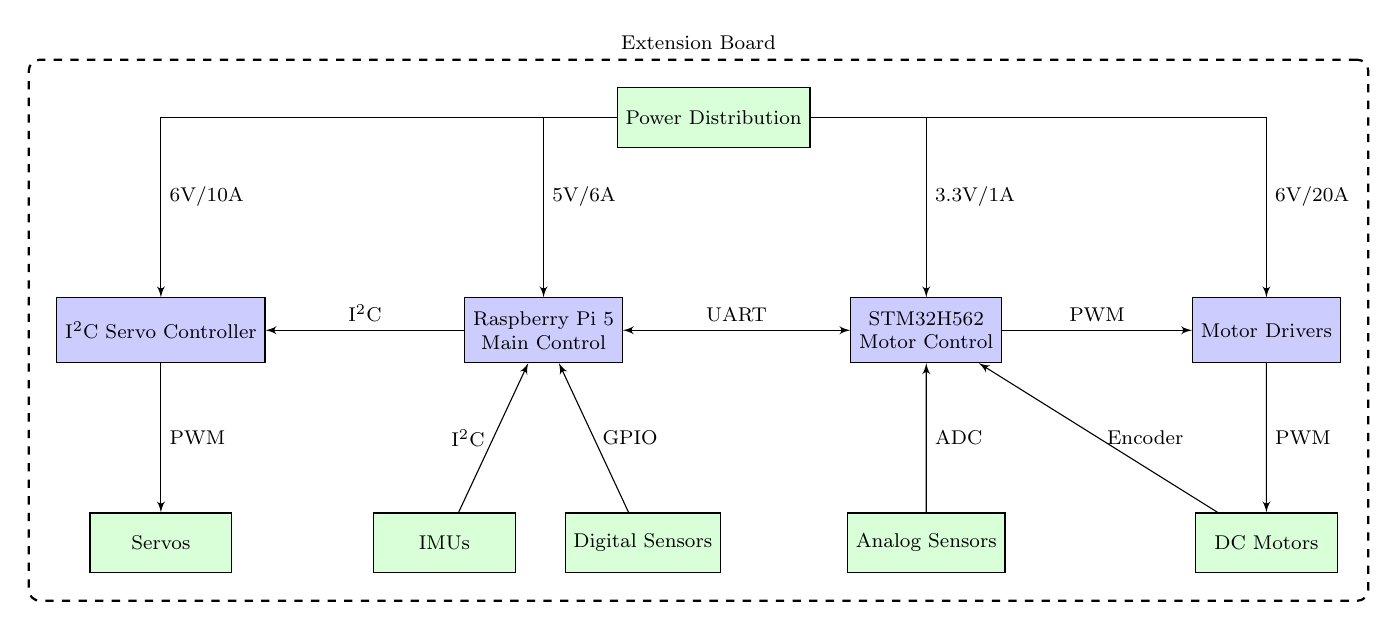
\begin{tikzpicture}[auto, font=\footnotesize, scale=0.9, transform shape]
		\tikzstyle{block} = [draw, fill=blue!20, rectangle,
		minimum height=2.6em, minimum width=2cm, align=center]
		\tikzstyle{io} = [draw, fill=green!15, rectangle,
		minimum height=2.4em, minimum width=2cm, align=center]
		\tikzstyle{line} = [draw, -latex']
		\tikzstyle{boardbox} = [draw, rounded corners, thick, dashed, inner sep=0.35cm]
		\node [io] (power) at (7.8,3.0) {Power Distribution};
		\node [io] (imu) at (4,-3.0) {IMUs};
		\node [block] (rpi) at (5.4,0) {Raspberry Pi 5\\Main Control};
		\node [block] (stm) at (10.8,0) {STM32H562\\Motor Control};
		\node [block] (motor) at (15.6,0) {Motor Drivers};
		\node [io] (motors) at (15.6,-3.0) {DC Motors};
		\node [block] (servoctl) at (0,0) {I\textsuperscript{2}C Servo Controller};
		\node [io] (digital) at (6.8,-3.0) {Digital Sensors};
		\node [io] (analog) at (10.8,-3.0) {Analog Sensors};
		\node [io] (servos) at (0,-3.0) {Servos};

		\draw [line] (power) -| node[pos=0.72, right] {5V/6A} (rpi);
		\draw [line] (power) -| node[pos=0.72, right] {3.3V/1A} (stm);
		\draw [line] (power) -| node[pos=0.72, right] {6V/20A} (motor);
		\draw [line] (power) -| node[pos=0.72, right] {6V/10A} (servoctl);
		\draw [line] (imu) -- node[left] {I\textsuperscript{2}C} (rpi);
		\draw [<->, >=latex'] (rpi) -- node[above] {UART} (stm);
		\draw [line] (stm) -- node[above] {PWM} (motor);
		\draw [line] (motor) -- node[right] {PWM} (motors);
		\draw [line] (motors) -- node[right] {Encoder} (stm);
		\draw [line] (servoctl) -- node[right] {PWM} (servos);
		\draw [line] (rpi) -- node[above] {I\textsuperscript{2}C} (servoctl);
		\draw [line] (digital) -- node[right] {GPIO} (rpi);
		\draw [line] (analog) -- node[right] {ADC} (stm);
		\begin{scope}[on background layer]
			\node [boardbox, fit=(power) (imu) (rpi) (stm) (motor) (servoctl),
			label={[align=center]above:Extension Board}] {};
		\end{scope}
	\end{tikzpicture}
	\caption{Funktionales Blockschaltbild des geplanten Gesamtsystems}
\end{figure}

\section{Hardwareentwurf und Bauteilauswahl}
\subsection{Raspberry-Pi-Anbindung}
Der Raspberry Pi 5 bildet die zentrale Recheneinheit des Systems. Die Erweiterungsplatine stellt die benötigten Signale und Versorgungen über die GPIO-Schnittstelle bereit. Dadurch lassen sich Steuerdaten, Kommunikationsschnittstellen und Hilfssignale direkt mit den Baugruppen auf der Platine verbinden.

Die Wahl des Raspberry Pi 5 erfolgte wegen der im Vergleich zu früheren Lösungen höheren Rechenleistung, der guten Linux-Unterstützung und der Verfügbarkeit im schulischen Umfeld. Für Robotikanwendungen mit Kamera, Bildverarbeitung oder später auch KI-gestützten Auswerteverfahren bietet diese Plattform genügend Reserven. Zusätzlich kann ein externer KI-Beschleuniger angebunden werden, welcher in diesem Fall der Raspberry Pi AI HAT+ (26 TOPS) ist.

\subsection{Spannungsversorgung}
Die Platine wird über einen 12-V-Eingang versorgt, der zu einem 3S1P-Akkusystem passt. Aus dieser Spannung werden mehrere niedrigere Versorgungsspannungen erzeugt.

Der Entwurf enthält drei 6-V-Versorgungsbereiche sowie eine 5-V-Versorgung für den Raspberry Pi. Aus der 5-V-Schiene wird zusätzlich eine 3,3-V-Versorgung für Logik und Peripherie erzeugt. Diese Aufteilung reduziert Wirkungen von Motoren und Servos auf den Logikbereich.

Bei der Auswahl der Spannungswandler stand die Stromtragfähigkeit im Vordergrund. Insbesondere für den Raspberry Pi und die Servoversorgung mussten ausreichende Reserven vorgesehen werden. Getrennte Versorgungspfade sind erforderlich, weil im Robotikbetrieb kurzzeitig hohe Ströme und Lastwechsel auftreten können.

\subsection{Motoransteuerung}
Die DC-Motoren werden über eigene Treiberstufen angesteuert. Im vorliegenden Entwurf kommen dafür drei DRV8411-Bausteine zum Einsatz. Sie übernehmen die leistungsseitige Ansteuerung, während die Steuersignale vom Mikrocontroller erzeugt werden.

Der STM32H562RIT6 wurde als Motor- und Echtzeitcontroller gewählt, weil er mehrere Timer mit PWM-Kanälen, ADC-Eingänge und UART bereitstellt. Dadurch kann er die zeitkritische Motoransteuerung, Encoder-Auswertung und analoge Signalerfassung übernehmen, während der Raspberry Pi die übergeordnete Logik ausführt.

\subsection{Servoansteuerung}
Für Servomotoren wurde ein eigener Versorgungs- und Anschlussbereich vorgesehen. Die eigentliche Signalerzeugung erfolgt über den PCA9685, der direkt vom Raspberry Pi angesteuert wird. Dieser Baustein erlaubt viele PWM-Ausgänge über eine I\textsuperscript{2}C-Schnittstelle zu steuern. Dadurch bleibt die Servoansteuerung vom STM32-Teil getrennt.

\subsection{Sensoranschlüsse}
Das Board bietet Anschlüsse für digitale und analoge Sensoren. Analoge Signale werden über den STM32 erfasst, da der Raspberry Pi keine eigenen ADC-Kanäle besitzt. Ein Teil dieser Kanäle ist differenziell ausgelegt. Digitale Sensoren können direkt durch den Raspberry Pi ausgewertet werden.

\subsection{Inertialsensoren}
Auf dem Board sind zwei IMUs vorgesehen: der BNO085 und der LSM6DSO.  Der BNO085 eignet sich besonders für orientierungsbezogene Auswertung, während der LSM6DSO eine zweite Messbasis liefert. Die IMUs werden direkt an den Raspberry Pi angebunden und nicht über den STM32 verarbeitet.

\section{PCB-Design und Layout}
Dieser Abschnitt beschreibt die praktische Umsetzung des Schaltplans auf der Leiterplatte. Im Gegensatz zum vorherigen Kapitel geht es hier nicht mehr um die Auswahl einzelner Bauteile, sondern um deren Platzierung, Verschaltung und elektrische Trennung im Layout.

Nach dem Schaltplanentwurf wurde das Layout der Leiterplatte erstellt. Dabei war es wichtig, die stromstarken Bereiche von den empfindlichen Logik- und Sensorschaltungen zu trennen. Die Bauteile wurden so platziert, dass die Stromversorgung kurze Wege zu den Verbrauchern hat und zusammengehörige Funktionsgruppen nah beieinander liegen.

Ein Schwerpunkt lag auf einer klaren Trennung zwischen Leistungsteil und Logikbereich sowie auf einer praktikablen Anordnung der Steckverbinder. Auch die Leitungsführung rund um den STM32 wurde so ausgelegt, dass die wichtigsten Signale möglichst direkt und übersichtlich geführt werden.


\begin{figure}[H]
	\centering
	\begin{tikzpicture}
		\node[anchor=south west, inner sep=0] (board) at (0,0)
		{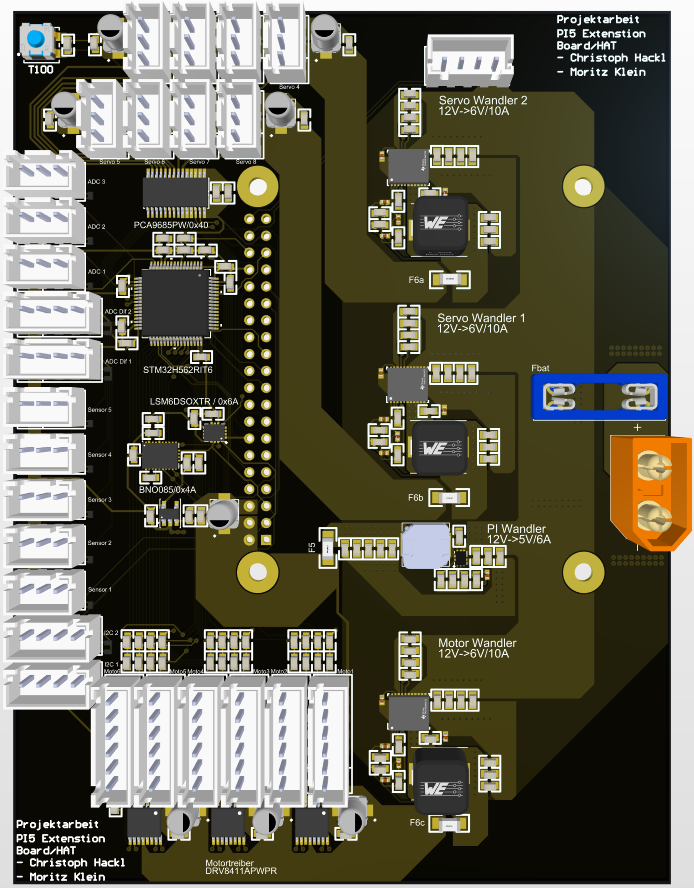
\includegraphics[width=0.92\linewidth]{Board.png}};
		\begin{scope}[x={(board.south east)}, y={(board.north west)}]
			\draw[red, very thick, fill=red!20, fill opacity=0.18]
			(0.53,0.05) rectangle (0.90,0.90);
			\node[draw=red, fill=white, rounded corners=2pt, font=\scriptsize, align=center]
			at (0.84,0.88) {Spannungs-\\wandler};

			\draw[blue, very thick, fill=blue!20, fill opacity=0.18]
			(0.15,0.38) rectangle (0.35,0.82);
			\node[draw=blue, fill=white, rounded corners=2pt, font=\scriptsize, align=center]
			at (0.25,0.66) {STM32 /\\Logik};

			\draw[green!50!black, very thick, fill=green!30, fill opacity=0.18]
			(0.09,0.82) rectangle (0.53,1);
			\node[draw=green!50!black, fill=white, rounded corners=2pt, font=\scriptsize, align=center]
			at (0.49,0.84) {Servo-\\bereich};

			\draw[orange, very thick, fill=orange!30, fill opacity=0.18]
			(0.15,0.00) rectangle (0.53,0.29);
			\node[draw=orange, fill=white, rounded corners=2pt, font=\scriptsize, align=center]
			at (0.33,0.31) {Motor-\\treiber};

			\draw[violet, very thick, fill=violet!25, fill opacity=0.18]
			(0.77,0.38) rectangle (1,0.58);
			\node[draw=violet, fill=white, rounded corners=2pt, font=\scriptsize, align=center]
			at (0.82,0.45) {Akku-\\eingang};

			\draw[cyan!60!black, very thick, fill=cyan!25, fill opacity=0.16]
			(0.00,0.20) rectangle (0.15,0.82);
			\node[draw=cyan!60!black, fill=white, rounded corners=2pt, font=\scriptsize, align=center]
			at (0.07,0.18) {Sensor-\\anschlüsse};

			\draw[magenta!80!black, very thick, fill=magenta!35, fill opacity=0.20]
			(0.35,0.38) rectangle (0.40,0.76);
			\node[draw=magenta!80!black, fill=white, rounded corners=2pt, font=\scriptsize, align=center]
			at (0.46,0.58) {Raspberry-\\Pi-Header};
		\end{scope}
	\end{tikzpicture}
	\caption{PCB-Layout mit markierten Spannungs- und Logikbereichen}
\end{figure}

\section{Fertigung, Bestückung und Inbetriebnahme}
Nach Abschluss des Layouts wurden Fertigungsdaten erzeugt, die Platine bestellt und bestückt. In der ersten Inbetriebnahme stand die grundlegende elektrische Funktionsprüfung im Vordergrund. Ziel dieser Phase war es, die Versorgung, die Erreichbarkeit der zentralen Komponenten und offensichtliche Hardwarefehler früh zu prüfen.

Die folgende Tabelle fasst den aktuellen Stand der Inbetriebnahme zusammen. Dabei handelt es sich um Funktionsprüfungen und grobe Spannungsprüfungen, noch nicht um eine vollständige messtechnische Charakterisierung.

\begin{table}[H]
	\centering
	\small
	\renewcommand{\arraystretch}{1.35}
	\begin{tabularx}{\linewidth}{>{\RaggedRight\arraybackslash}m{0.22\linewidth}|>{\RaggedRight\arraybackslash}m{0.29\linewidth}|>{\RaggedRight\arraybackslash}m{0.25\linewidth}|>{\Centering\arraybackslash}m{0.11\linewidth}}
		\hline
		\textbf{Teilbereich} & \textbf{Prüfung} & \textbf{Ergebnis} & \textbf{Status} \\\hline
		Spannungsversorgung & Kontrolle der erzeugten Versorgungsschienen & 6-V-Bereiche liefern ca. 6 V, Raspberry-Pi-Schiene ca. 5 V, Logikversorgung ca. 3,3 V & funktioniert \\\hline
		STM32 & Programmieren und Erreichen des Mikrocontrollers über SWD & STM32 kann geflasht werden & funktioniert \\\hline
		Motoransteuerung & STM32 setzt PWM-Signale an den Motortreibern & Motortreiber reagieren auf die vom STM32 ausgegebenen Steuersignale & funktioniert \\\hline
		UART-Kommunikation & Steuerbefehle vom Raspberry Pi beziehungsweise Testsystem an den STM32 & UART-Kommandos können verarbeitet und in PWM-Werte umgesetzt werden & funktioniert \\\hline
		IMU LSM6DSO & Zugriff vom Raspberry Pi über die verwendete Softwarebibliothek & Sensor ist erreichbar und kann angesprochen werden & funktioniert \\\hline
		IMU BNO085 & Zugriff vom Raspberry Pi über die verwendete Softwarebibliothek & Sensor ist derzeit nicht erreichbar & offen \\\hline
		Servoansteuerung & Ansteuerung des PCA9685 und Prüfung des PWM-Ausgangs & Gewünschtes PWM-Signal wird erzeugt & funktioniert \\\hline
	\end{tabularx}
	\caption{Aktueller Stand der Inbetriebnahme}
\end{table}


\section{Fehler, Probleme und bereits umgesetzte Verbesserungen}
\subsection{Fehler im Schaltplan aus dem Power-Designer}
Ein konkreter Fehler trat bei der Übernahme eines Schaltungsteils aus dem Texas-Instruments-Power-Designer auf. Beim Abzeichnen der erzeugten Schematic wurde ein Fehler übernommen, der erst im späteren Verlauf erkannt wurde.

Die Korrektur erfolgte direkt an der aufgebauten Platine durch das Auftrennen einer Leiterbahn. Damit konnte der Fehler behoben werden. Für eine nächste Platinenrevision muss diese Änderung jedoch sauber in Schaltplan und Layout zurückgeführt werden.

\subsection{Empfindlichkeit des 5-V-Wandlers beim Abziehen des Akkus}
Ein weiteres Problem betrifft den 5-V-Wandler für den Raspberry Pi. Wenn der Akku während des Betriebs einfach abgezogen wird, kann der Wandler beschädigt werden. Deshalb darf der Akku derzeit nur getrennt werden, nachdem der Raspberry Pi sauber heruntergefahren und abgeschaltet wurde.

Für eine zukünftige Revision sollte daher geprüft werden, ob zusätzliche Schutzmaßnahmen, ein geänderter Abschaltpfad oder eine robustere Wandlerlösung notwendig sind.


\section{Firmware des STM32-Mikrocontrollers}
\subsection{Rolle des Mikrocontrollers}
Der STM32 ist als echtzeitfähiger Co-Prozessor des Raspberry Pi vorgesehen. Er soll später die hardwarenahen Aufgaben übernehmen, insbesondere PWM-Ausgabe, ADC-Erfassung und die Kommunikation mit dem Raspberry Pi.

\subsection{Aktueller Stand der Firmware}
Im aktuellen Projektstand ist die Grundkonfiguration des Mikrocontrollers bereits in STM32CubeIDE angelegt. Dazu gehören:

\begin{itemize}
	\item Auslesen analoger Sensoren über den ADC
	\item Ansteuerung von Motoren über PWM
	\item Kommunikation mit dem Raspberry Pi über UART
	\item Rückmeldung von Zustands- und Sensordaten an den Raspberry Pi
\end{itemize}

\subsection{Ablauf des aktuellen STM32-Programms}
Der aktuelle Ablauf: Nach der Initialisierung der HAL, des Systemtakts und der Peripherie werden die PWM-Ausgänge gestartet, alle Motoren zunächst auf Freilauf gesetzt und die Anfangszustände der Encoder gespeichert. Danach läuft das Programm dauerhaft in einer Hauptschleife.

\begin{figure}[H]
	\centering
	\resizebox{\textwidth}{!}{%
	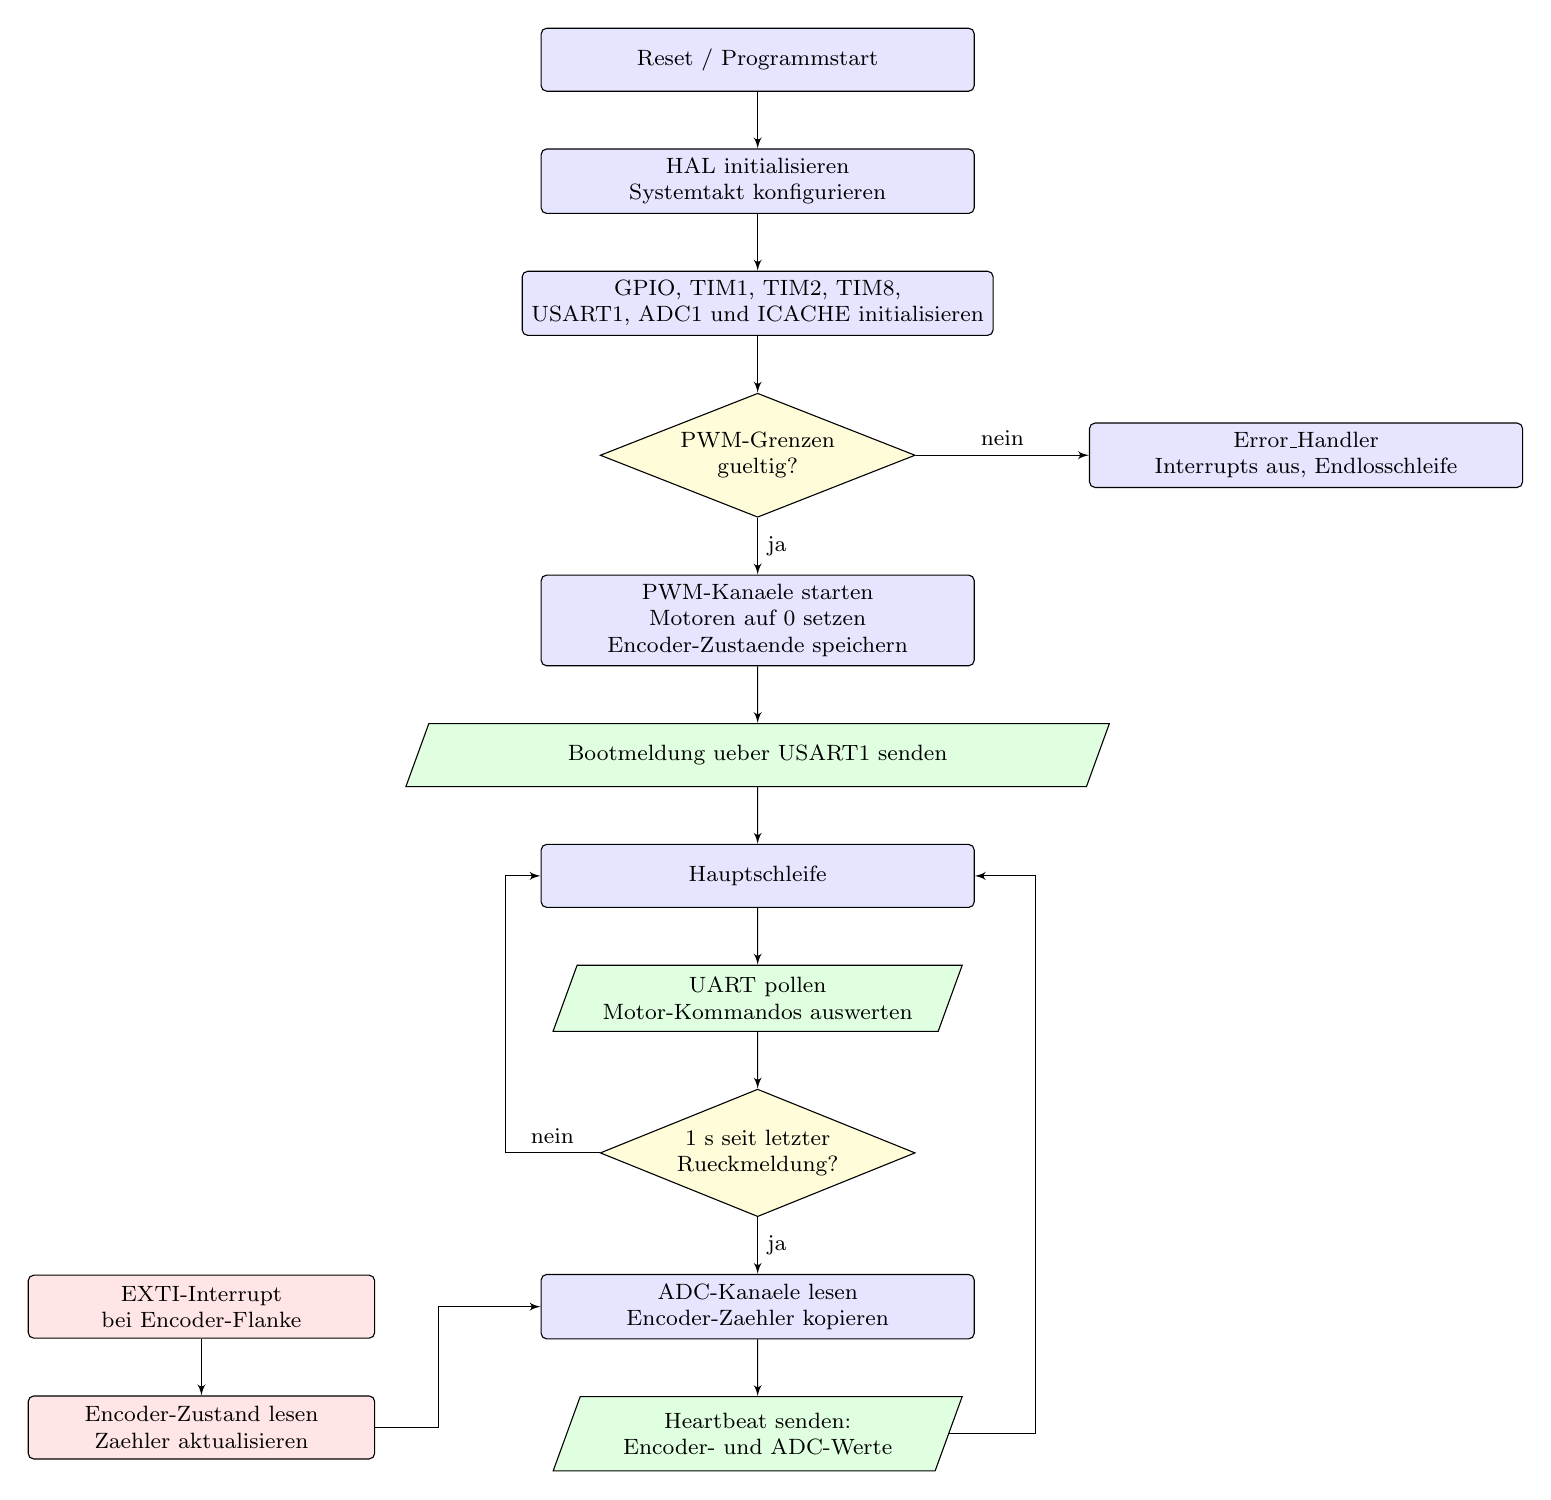
\begin{tikzpicture}[
		font=\footnotesize,
		node distance=0.72cm,
		process/.style={draw, rectangle, rounded corners=2pt, align=center, minimum width=5.5cm, minimum height=0.8cm, fill=blue!10},
		decision/.style={draw, diamond, aspect=2.2, align=center, inner sep=1pt, minimum width=4.0cm, fill=yellow!15},
		io/.style={draw, trapezium, trapezium left angle=70, trapezium right angle=110, align=center, minimum width=5.2cm, minimum height=0.8cm, fill=green!12},
		interrupt/.style={draw, rectangle, rounded corners=2pt, align=center, minimum width=4.4cm, minimum height=0.8cm, fill=red!10},
		line/.style={draw, -latex'}
	]
		\node[process] (start) {Reset / Programmstart};
		\node[process, below=of start] (hal) {HAL initialisieren\\Systemtakt konfigurieren};
		\node[process, below=of hal] (peripherals) {GPIO, TIM1, TIM2, TIM8,\\USART1, ADC1 und ICACHE initialisieren};
		\node[decision, below=of peripherals] (pwmcheck) {PWM-Grenzen\\gueltig?};
		\node[process, right=2.2cm of pwmcheck] (error) {Error\_Handler\\Interrupts aus, Endlosschleife};
		\node[process, below=of pwmcheck] (startup) {PWM-Kanaele starten\\Motoren auf 0 setzen\\Encoder-Zustaende speichern};
		\node[io, below=of startup] (bootmsg) {Bootmeldung ueber USART1 senden};
		\node[process, below=of bootmsg] (loop) {Hauptschleife};
		\node[io, below=of loop] (uart) {UART pollen\\Motor-Kommandos auswerten};
		\node[decision, below=of uart] (tick) {1 s seit letzter\\Rueckmeldung?};
		\node[process, below=of tick] (read) {ADC-Kanaele lesen\\Encoder-Zaehler kopieren};
		\node[io, below=of read] (send) {Heartbeat senden:\\Encoder- und ADC-Werte};
		\node[interrupt, left=2.1cm of read] (exti) {EXTI-Interrupt\\bei Encoder-Flanke};
		\node[interrupt, below=of exti] (encupdate) {Encoder-Zustand lesen\\Zaehler aktualisieren};

		\draw[line] (start) -- (hal);
		\draw[line] (hal) -- (peripherals);
		\draw[line] (peripherals) -- (pwmcheck);
		\draw[line] (pwmcheck) -- node[above] {nein} (error);
		\draw[line] (pwmcheck) -- node[right] {ja} (startup);
		\draw[line] (startup) -- (bootmsg);
		\draw[line] (bootmsg) -- (loop);
		\draw[line] (loop) -- (uart);
		\draw[line] (uart) -- (tick);
		\draw[line] (tick) -- node[right] {ja} (read);
		\draw[line] (read) -- (send);
		\draw[line] (send.east) -- ++(1.1,0) |- (loop.east);
		\draw[line] (tick.west) -- node[above] {nein} ++(-1.2,0) |- (loop.west);
		\draw[line] (exti) -- (encupdate);
		\draw[line] (encupdate.east) -- ++(0.8,0) |- (read.west);
	\end{tikzpicture}
	}
	\caption{Programmablauf der aktuellen STM32-Firmware}
\end{figure}

\subsection{UART-Kommunikationsprotokoll}
Die Kommunikation zwischen Raspberry Pi und STM32 erfolgt im aktuellen Firmwarestand über USART1 mit 115200 Baud, 8 Datenbits, keiner Parität und einem Stoppbit. Diese Geschwindigkeit ist für die geplanten Steuerbefehle und Statusdaten ausreichend, da nur kurze Textnachrichten übertragen werden.

Kommandos vom Raspberry Pi werden zeichenweise eingelesen. Der Empfangspuffer ist 64 Byte groß. Ein Motorbefehl beginnt mit \texttt{M} und enthält anschließend bis zu sechs Prozentwerte für die Motoren. Leerzeichen, Tabulatoren, Kommas und Semikolons können als Trennzeichen verwendet werden. Die Werte werden im STM32 auf den Bereich von -100 bis 100 begrenzt und danach auf die PWM-Tastverhältnisse umgerechnet.

\begin{codeblock}
M 20 -10 0 0 50 -50
\end{codeblock}

Die Rückmeldung vom STM32 erfolgt einmal pro Sekunde. Dabei werden zuerst die sechs Encoderzähler und danach die fünf ADC-Werte übertragen. Das Format ist als einfache ASCII-Zeile aufgebaut und kann auf dem Raspberry Pi ohne großen Aufwand geparst werden.

\begin{codeblock}
ENC 120 118 0 0 -34 -31 ADC 2048 2011 1995 1020 980
\end{codeblock}

Zusätzlich sendet der STM32 nach dem Start eine kurze Bootmeldung. Damit kann der Raspberry Pi erkennen, dass die Firmware gestartet ist und die PWM-Ausgänge initialisiert wurden.

\subsection{Programmierung über SWD}
Beim ursprünglich geplanten Flashen des STM32 über den USART-Bootloader zeigte sich ein Problem: Der Bootloader unterstützt USART nur auf festgelegten Pins. Nach AN2606, Abschnitt 57.1 und Tabelle 127, liegen die dafür vorgesehenen Pins beim STM32H562xx für USART1 auf PA9/PA10, für USART2 auf PA2/PA3 und für USART3 auf PD8/PD9. Diese Pinbelegung stimmt nicht mit den ursprünglich für den Boot- und Flash-Vorgang geplanten Pins überein.

Deshalb wird der STM32 nun über SWD programmiert und debuggt. UART bleibt weiterhin erhalten, wird aber nur für die Kommunikation zwischen Raspberry Pi und STM32 verwendet. Für die geplanten Steuerbefehle und Statusdaten ist UART schnell genug und reduziert den Aufwand für das Kommunikationsprotokoll.



\section{Geplante Messungen und Auswertungen}
Bereits in der Projektarbeitsanfrage wurden konkrete Messungen für das fertige System vorgesehen. Diese betreffen einerseits die Stromversorgung und andererseits die Aktorik sowie die Rückführung über Encoder. Auch wenn zum aktuellen Stand noch nicht alle Messwerte vorliegen, soll dieser Abschnitt den geplanten technischen Aufbau und die Auswertungssystematik dokumentieren.

Die in der Antragsphase verwendete Bezeichnung \glqq ESP\grqq{} bezieht sich auf den damals vorgesehenen Mikrocontrollerteil. Im aktuellen Entwicklungsstand wird diese Funktion durch den STM32 übernommen. Die geplanten Messungen bleiben inhaltlich jedoch gleich.

\subsection{Messungen an den Powerrails}
Die Stromversorgung ist ein zentrales Teilsystem der gesamten Platine. Deshalb müssen die einzelnen Versorgungsschienen nicht nur auf ihre Sollspannung, sondern auch auf ihr Verhalten unter Last untersucht werden. Laut Projektantrag stehen dabei insbesondere Spannung und Strom unter Last, Leistungsaufnahme, Wirkungsgrad und Stabilität im Vordergrund.

\subsubsection{Messziel}
Mit diesen Messungen soll überprüft werden,

\begin{itemize}
	\item ob die einzelnen Versorgungsschienen ihre Sollspannungen einhalten,
	\item wie groß die Stromentnahme unter verschiedenen Lastfällen ist,
	\item wie hoch die resultierende Leistungsaufnahme ausfällt,
	\item wie effizient die Umwandlung von 12\,V auf 6\,V, 5\,V und 3,3\,V erfolgt,
	\item ob es beim Zu- oder Abschalten zu kritischen Einbrüchen, Überschwingern oder Instabilitäten kommt.
\end{itemize}

\subsubsection{Messaufbau}
Als Spannungsquelle wird ein Labornetzteil oder der vorgesehene Akku mit bekannter Eingangsspannung verwendet. Die jeweilige Ausgangsschiene wird anschließend mit einer definierten Last beaufschlagt. Je nach Messung können dafür Lastwiderstände, elektronische Lasten oder die real angeschlossenen Verbraucher verwendet werden.

Gemessen werden:

\begin{itemize}
	\item Eingangsspannung und Eingangsstrom des Wandlers
	\item Ausgangsspannung und Ausgangsstrom der jeweiligen Schiene
	\item eventuelle Spannungseinbrüche beim Lastwechsel
	\item Schaltverhalten beim Ein- und Ausschalten
\end{itemize}

Die Messwerte sollen später einheitlich in einer Tabelle erfasst werden. Wichtig ist dabei, nicht nur die Leerlaufspannung, sondern auch das Verhalten unter Last zu dokumentieren.

\begin{figure}[H]
	\centering
	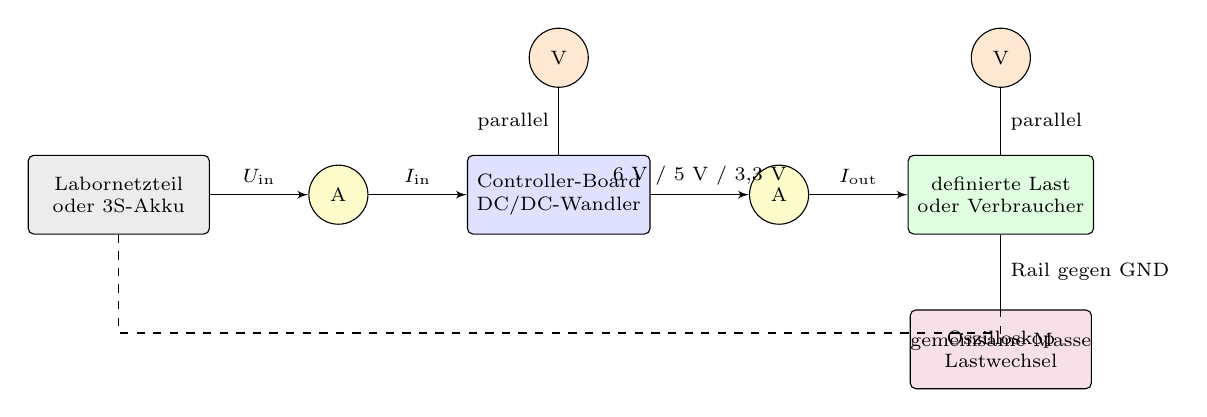
\begin{tikzpicture}[font=\scriptsize, node distance=1.25cm, >=latex]
		\tikzstyle{block} = [draw, rectangle, rounded corners=2pt, minimum height=1.0cm, minimum width=2.3cm, align=center]
		\tikzstyle{meter} = [draw, circle, minimum size=0.75cm, align=center]
		\tikzstyle{line} = [draw, -latex']

		\node[block, fill=gray!15] (source) {Labornetzteil\\oder 3S-Akku};
		\node[meter, fill=yellow!20, right=of source] (ain) {A};
		\node[block, fill=blue!12, right=of ain] (board) {Controller-Board\\DC/DC-Wandler};
		\node[meter, fill=yellow!20, right=of board] (aout) {A};
		\node[block, fill=green!12, right=of aout] (load) {definierte Last\\oder Verbraucher};
		\node[meter, fill=orange!18, above=0.85cm of board] (vin) {V};
		\node[meter, fill=orange!18, above=0.85cm of load] (vout) {V};
		\node[block, fill=purple!12, below=0.95cm of load] (scope) {Oszilloskop\\Lastwechsel};

		\draw[line] (source) -- node[above] {$U_\mathrm{in}$} (ain);
		\draw[line] (ain) -- node[above] {$I_\mathrm{in}$} (board);
		\draw[line] (board) -- node[above] {6 V / 5 V / 3,3 V} (aout);
		\draw[line] (aout) -- node[above] {$I_\mathrm{out}$} (load);
		\draw[draw] (vin) -- node[left] {parallel} (board);
		\draw[draw] (vout) -- node[right] {parallel} (load);
		\draw[draw] (scope) -- node[right] {Rail gegen GND} (load);
		\draw[draw, dashed] (source.south) |- ++(0,-1.25) -| node[pos=0.55, below] {gemeinsame Masse} (load.south);
	\end{tikzpicture}
	\caption{Messaufbau zur Überprüfung der Powerrails}
\end{figure}

\begin{table}[H]
	\centering
	\scriptsize
	\renewcommand{\arraystretch}{1.25}
	\setlength{\tabcolsep}{3pt}
	\begin{tabularx}{\linewidth}{L{0.16\linewidth}|L{0.12\linewidth}|L{0.14\linewidth}|L{0.14\linewidth}|L{0.12\linewidth}|L{0.15\linewidth}}
		\hline
		\textbf{Schiene} & \textbf{Sollwert} & \textbf{Leerlauf} & \textbf{unter Last} & \textbf{Laststrom} & \textbf{Bewertung} \\\hline
		6 V Motor & 6 V &  &  &  &  \\\hline
		6 V Servo & 6 V &  &  &  &  \\\hline
		5 V Raspberry Pi & 5 V &  &  &  &  \\\hline
		3,3 V Logik & 3,3 V &  &  &  &  \\\hline
	\end{tabularx}
	\caption{Vorgesehene Messwerttabelle für die Powerrails}
\end{table}

\subsubsection{Messschaltung}
Die Strommessung kann entweder über das Labornetzteil, ein Multimeter in Serie oder einen niederohmigen Shunt-Widerstand mit Spannungsabfallmessung erfolgen. Die Spannungsmessung erfolgt direkt an den Testpunkten der jeweiligen Powerrail. Für das Beobachten von Einbrüchen oder Schaltspitzen ist zusätzlich ein Oszilloskop sinnvoll.

\subsubsection{Auswertung und Interpretation}
Aus den gemessenen Größen lassen sich Eingangsleistung, Ausgangsleistung und Wirkungsgrad berechnen. Außerdem kann beurteilt werden, ob die Spannungsversorgung für die jeweilige Last ausreichend stabil ist. Besonders wichtig ist dabei die Bewertung unter realistischen Lastbedingungen.

Für das vorliegende Projekt ist diese Messung besonders relevant, weil bereits ein reales Problem beim 5-V-Wandler beobachtet wurde. Das Verhalten beim Abziehen des Akkus beziehungsweise beim Abschalten der Versorgung muss deshalb besonders kritisch betrachtet werden.

\subsection{Messungen an den Encodersignalen}
Die Encoder dienen als Rückführung für die spätere Motorregelung. Daher müssen nicht nur die elektrischen Signale selbst, sondern auch deren Qualität und Auswertbarkeit untersucht werden.

\subsubsection{Messziel}
Bei den Encodermessungen soll überprüft werden,

\begin{itemize}
	\item ob die Signale elektrisch sauber und störungsarm vorliegen,
	\item ob die Impulsfolge zur tatsächlichen Bewegung passt,
	\item ob sich die Drehrichtung eindeutig erkennen lässt,
	\item ob die Auflösung und Genauigkeit für die geplante Regelung ausreichend sind.
\end{itemize}

\subsubsection{Messaufbau}
Ein Motor mit angeschlossenem Encoder wird kontrolliert betrieben. Die Encodersignale werden gleichzeitig am Mikrocontroller-Eingang und gegebenenfalls direkt am Stecker oder an einem Testpunkt gemessen. Dabei kann der Motor mit verschiedenen Drehzahlen und in beiden Drehrichtungen betrieben werden.

Zur Untersuchung eignen sich vor allem:

\begin{itemize}
	\item Oszilloskop zur Darstellung der Encoderkanäle
	\item Logikanalysator zur Impulszählung und Richtungsanalyse
	\item Vergleich mit einer bekannten mechanischen Bewegung oder Umdrehungszahl
\end{itemize}

Die Ergebnisse sollen sowohl elektrisch als auch funktional bewertet werden. Neben den Pegeln ist vor allem wichtig, ob die Flanken sauber erkannt werden und ob die Drehrichtung korrekt aus Kanal A und Kanal B abgeleitet werden kann.

\begin{figure}[H]
	\centering
	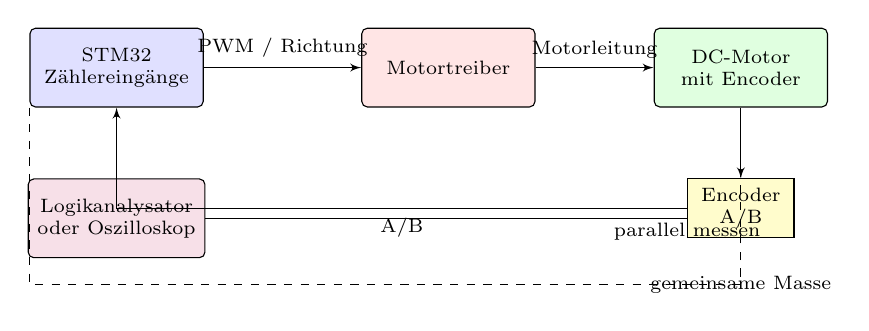
\begin{tikzpicture}[font=\scriptsize, node distance=1.1cm, >=latex]
		\tikzstyle{block} = [draw, rectangle, rounded corners=2pt, minimum height=1.0cm, minimum width=2.2cm, align=center]
		\tikzstyle{signal} = [draw, rectangle, minimum height=0.65cm, minimum width=1.35cm, align=center]
		\tikzstyle{line} = [draw, -latex']

		\node[block, fill=blue!12] (stm) {STM32\\Zählereingänge};
		\node[block, fill=red!10, right=2.0cm of stm] (driver) {Motortreiber};
		\node[block, fill=green!12, right=1.5cm of driver] (motor) {DC-Motor\\mit Encoder};
		\node[signal, fill=yellow!20, below=0.9cm of motor] (enc) {Encoder\\A/B};
		\node[block, fill=purple!12, below=0.9cm of stm] (logic) {Logikanalysator\\oder Oszilloskop};

		\draw[line] (stm) -- node[above] {PWM / Richtung} (driver);
		\draw[line] (driver) -- node[above] {Motorleitung} (motor);
		\draw[line] (motor) -- (enc);
		\draw[line] (enc.west) -| node[pos=0.25, below] {A/B} (stm.south);
		\draw[draw] (enc.west) |- node[pos=0.25, below] {parallel messen} (logic.east);
		\draw[draw, dashed] (stm.south west) |- ++(0,-2.25) -| node[pos=0.55, below] {gemeinsame Masse} (motor.south);
	\end{tikzpicture}
	\caption{Messaufbau zur Prüfung der Encodersignale}
\end{figure}

\begin{table}[H]
	\centering
	\scriptsize
	\renewcommand{\arraystretch}{1.25}
	\setlength{\tabcolsep}{3pt}
	\begin{tabularx}{\linewidth}{L{0.17\linewidth}|L{0.14\linewidth}|L{0.14\linewidth}|L{0.16\linewidth}|L{0.23\linewidth}}
		\hline
		\textbf{Messpunkt} & \textbf{Pegel} & \textbf{Frequenz} & \textbf{Phasenlage} & \textbf{Bewertung} \\\hline
		Encoder 1 A/B &  &  &  &  \\\hline
		Encoder 2 A/B &  &  &  &  \\\hline
		Encoder 3 A/B &  &  &  &  \\\hline
		Encoder 4 A/B &  &  &  &  \\\hline
		Encoder 5 A/B &  &  &  &  \\\hline
		Encoder 6 A/B &  &  &  &  \\\hline
	\end{tabularx}
	\caption{Vorgesehene Messwerttabelle für die Encodersignale}
\end{table}

\subsubsection{Messschaltung}
Die Encodersignale werden über die dafür vorgesehenen Leitungen an den Mikrocontroller geführt. Für die Messung werden diese Leitungen parallel an ein Oszilloskop oder einen Logikanalysator angeschlossen. Wichtig ist dabei eine gemeinsame Massebeziehung, damit die Signalform korrekt beurteilt werden kann.

\subsubsection{Auswertung und Interpretation}
Ausgewertet werden insbesondere Tastverhältnis, Signalpegel, Phasenlage der beiden Encoderkanäle und die Impulszahl pro Umdrehung. Die Phasenverschiebung zwischen den Kanälen gibt dabei Aufschluss über die Drehrichtung. Unscharfe Flanken, starke Störungen oder Pegelprobleme würden auf Schwachstellen in der Signalaufbereitung, Leitungsführung oder Pegelanpassung hinweisen.

\subsection{Messungen an Motoren und Servos}
Die dritte im Antrag vorgesehene Messgruppe betrifft Motoren und Servos selbst. Hier geht es in erster Linie um Stromaufnahme, Leistungsaufnahme und Verhalten unter Last.

\subsubsection{Messziel}
Mit diesen Messungen soll untersucht werden,

\begin{itemize}
	\item wie groß die Stromaufnahme der Motoren und Servos im Leerlauf und unter Last ist,
	\item welche Leistung im praktischen Betrieb benötigt wird,
	\item wie sich die Stromaufnahme bei Lastwechseln verändert,
	\item ob die vorhandenen Versorgungszweige ausreichend dimensioniert sind.
\end{itemize}

\subsubsection{Messaufbau}
Ein Motor beziehungsweise Servo wird an die reale Ausgangsstufe des Boards angeschlossen und anschließend in mehreren Betriebsfällen untersucht. Sinnvolle Lastfälle sind beispielsweise:

\begin{itemize}
	\item Leerlaufbetrieb
	\item Anlaufmoment
	\item Betrieb unter mechanischer Last
	\item blockierter oder nahezu blockierter Zustand für kurze kontrollierte Zeit
\end{itemize}

Gemessen werden dabei Strom, Spannung und gegebenenfalls das zeitliche Verhalten während des Einschaltens oder bei Lastsprüngen.

Die Messwerte sollen getrennt nach Motoren und Servos dokumentiert werden. Dadurch lässt sich später erkennen, ob die Auslegung der Treiber und der Versorgungszweige ausreichend Reserven besitzt.

\begin{figure}[H]
	\centering
	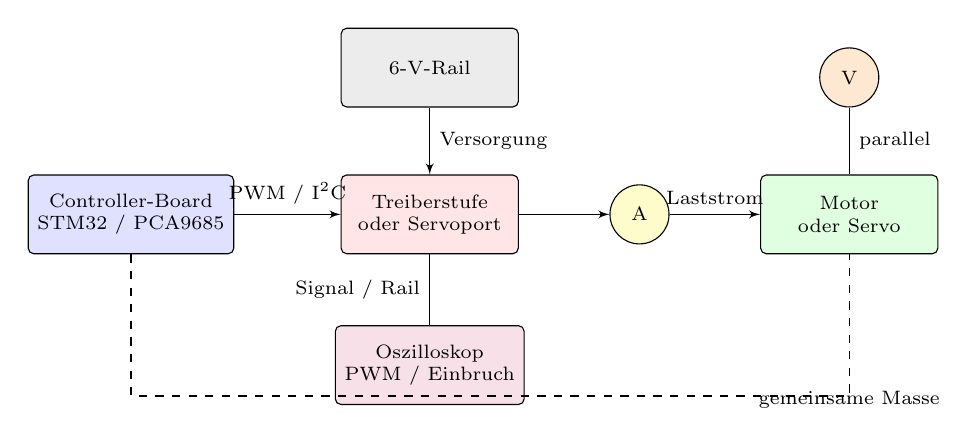
\begin{tikzpicture}[font=\scriptsize, node distance=1.05cm, >=latex]
		\tikzstyle{block} = [draw, rectangle, rounded corners=2pt, minimum height=1.0cm, minimum width=2.25cm, align=center]
		\tikzstyle{meter} = [draw, circle, minimum size=0.75cm, align=center]
		\tikzstyle{line} = [draw, -latex']

		\node[block, fill=blue!12] (board) {Controller-Board\\STM32 / PCA9685};
		\node[block, fill=red!10, right=1.35cm of board] (stage) {Treiberstufe\\oder Servoport};
		\node[meter, fill=yellow!20, right=1.15cm of stage] (amp) {A};
		\node[block, fill=green!12, right=1.15cm of amp] (load) {Motor\\oder Servo};
		\node[meter, fill=orange!18, above=0.85cm of load] (volt) {V};
		\node[block, fill=purple!12, below=0.9cm of stage] (scope) {Oszilloskop\\PWM / Einbruch};
		\node[block, fill=gray!15, above=0.85cm of stage] (rail) {6-V-Rail};

		\draw[line] (board) -- node[above] {PWM / I\textsuperscript{2}C} (stage);
		\draw[line] (rail) -- node[right] {Versorgung} (stage);
		\draw[line] (stage) -- (amp);
		\draw[line] (amp) -- node[above] {Laststrom} (load);
		\draw[draw] (volt) -- node[right] {parallel} (load);
		\draw[draw] (scope) -- node[left] {Signal / Rail} (stage);
		\draw[draw, dashed] (board.south) |- ++(0,-1.8) -| node[pos=0.55, below] {gemeinsame Masse} (load.south);
	\end{tikzpicture}
	\caption{Messaufbau für Motor- und Servomessungen}
\end{figure}

\begin{table}[H]
	\centering
	\scriptsize
	\renewcommand{\arraystretch}{1.25}
	\setlength{\tabcolsep}{3pt}
	\begin{tabularx}{\linewidth}{L{0.15\linewidth}|L{0.15\linewidth}|L{0.12\linewidth}|L{0.12\linewidth}|L{0.13\linewidth}|L{0.16\linewidth}}
		\hline
		\textbf{Verbraucher} & \textbf{Lastfall} & \textbf{Spannung} & \textbf{Strom} & \textbf{PWM / Signal} & \textbf{Bewertung} \\\hline
		DC-Motor & Leerlauf &  &  &  &  \\\hline
		DC-Motor & Anlauf &  &  &  &  \\\hline
		DC-Motor & Last &  &  &  &  \\\hline
		Servo & Ruheposition &  &  &  &  \\\hline
		Servo & Bewegung &  &  &  &  \\\hline
		Servo & Last &  &  &  &  \\\hline
	\end{tabularx}
	\caption{Vorgesehene Messwerttabelle für Motoren und Servos}
\end{table}

\subsubsection{Messschaltung}
Die Strommessung erfolgt wieder über ein in Serie geschaltetes Messgerät oder über einen Shunt. Die Spannung wird direkt am Verbraucher oder an den entsprechenden Versorgungsklemmen gemessen. Bei dynamischen Lasten bietet sich zusätzlich die Beobachtung mit dem Oszilloskop an, um kurze Stromspitzen oder Spannungseinbrüche sichtbar zu machen.

\subsubsection{Auswertung und Interpretation}
Die gemessenen Werte erlauben eine direkte Beurteilung der realen Belastung der einzelnen Powerrails. Daraus kann abgeleitet werden, ob Reserven vorhanden sind oder ob einzelne Bereiche thermisch beziehungsweise elektrisch kritisch werden können. Besonders relevant ist dabei das Verhalten bei Lastwechseln und kurzzeitigen Spitzen.

\subsection{Darstellung der Messungen in der finalen Dokumentation}
Sobald die Messungen praktisch durchgeführt wurden, sollten sie in der finalen Fassung jeweils einheitlich dokumentiert werden. Eine sinnvolle Struktur je Messung ist:

\begin{enumerate}
	\item Messziel
	\item verwendete Geräte
	\item Messaufbau und Messschaltung
	\item gemessene Werte in Tabelle oder Diagramm
	\item kurze fachliche Interpretation
\end{enumerate}

Dadurch entsteht ein nachvollziehbarer technischer Abschnitt, der nicht nur rohe Messwerte auflistet, sondern auch deren Bedeutung für das Gesamtsystem erklärt.

\section{Geplante Erweiterungen und nächste Schritte}
Aus dem bisherigen Entwicklungsstand ergeben sich mehrere konkrete Verbesserungen für die nächste Projektphase:

\begin{itemize}
	\item Verwendung der SWD-Schnittstelle für Programmierung und Debugging des STM32
	\item weitere Tests der UART-Kommunikation zwischen Raspberry Pi und STM32
	\item Überarbeitung kritischer Stellen im Layout
	\item genauere Analyse des 5-V-Wandlers und möglicher Schutzmaßnahmen
	\item weitere Ausarbeitung und Erprobung der eigentlichen STM32-Anwendungssoftware
\end{itemize}



\section{Fazit}
Mit dem Raspberry-Pi-Robotik-Controller wurde eine funktionsfähige Hardwareplattform für Robotikprojekte aufgebaut. Der bisherige Entwicklungsstand zeigt, dass das Grundkonzept tragfähig ist und die wichtigsten Funktionsbereiche auf einer gemeinsamen Platine zusammengeführt werden können.

Ebenso wichtig wie der aktuelle Stand sind die im Entwicklungsprozess erkannten Schwachstellen. Dazu zählen vor allem der Fehler im übernommenen Schaltungsteil, die Empfindlichkeit des 5-V-Wandlers beim Abziehen des Akkus sowie einzelne offene Punkte im Layout.

Die nächsten Schritte liegen in der weiteren Firmwareentwicklung und in den noch ausstehenden Messungen. Die SWD-Debugschnittstelle wird dafür als fester Programmier- und Debugzugang verwendet. Damit bildet die aktuelle Platine eine gute Basis für eine verbesserte nächste Revision.

\end{document}
